%%%%%%%%%%%%%%%%%%%%%%%%%%%%%%%%%%%%%%%%%%%%%%%%%%%%%%%%%%%%%%%%%%%%
% Diskussion und Ausblick
%%%%%%%%%%%%%%%%%%%%%%%%%%%%%%%%%%%%%%%%%%%%%%%%%%%%%%%%%%%%%%%%%%%%

\chapter{Discussion}
\label{discussion}
The re-implementation of Percolator in python works as intended. %Although concerns could be expressed that re-estimating the C parameter for every outer split might lead to overfitting, this is done by the original Percolator algorithm as well.
The slightly higher number of cross-linked PSMs found at $1\%$~q-value is likely due to randomness caused by differing splits and the wrong formula used for the calculating of q-values, as pointed out in~\ref{lab:background:bioinfo_tools}. The correct formula should be used for further usage of Pycolator.\\\\
As already explained in~\ref{lab:matmet:ranks}, scoring cross-linked peptides is often harder than scoring linear ones. Therefore, they can get a lower score than appropriate and it can be useful to also include the best scoring cross-linked peptide when running the Percolator algorithm. It may be able to revise the PSMs scores and the actually correct cross-linked peptide may become the best scoring PSM. This thesis is also supported by the findings in~\ref{lab:results:ranks}. If only including the best scoring peptide, of which~\ref{fig:only_rank_one} shows the results, the end result is worse than when giving Pycolator some iterations to re-rank the found PSMs. However, it was better than when giving Pycolator all of the PSMs available, which is unexpected, since giving a machine learning model more information should generally improve its learning. Apparently, the lower ranking PSMs, even when having such a high score that a q-value of $\leq5\%$ is estimated, contain misleading information and thus the SVM learns patterns not valid for correct PSMs. This also explains why the algorithm converges faster when only given rank 1 PSMs. The higher quality of data lets the SVM learn the correct patterns after fewer iterations. \\
The pseudo ROC generated when using the newly implemented mechanism~(\ref{fig:optimalranking}) shows a convergence after $5$ iterations, just like when using every PSM~(\ref{fig:all_ranks}). Then, as the log shows, lower ranking PSMs are dropped and the next iteration has a much higher AUC, probably as a result of the better quality of the PSMs. Letting the algorithm run on the new dataset again improves the AUC even beyond that of Pycolator when only using rank 1 PSMs. This suggests, that indeed a re-ranking takes place in the first half of iterations.\\
%Comparing the AUC of Pycolator when run with the new mechanism~(\ref{fig:optimalranking}) after iteration $6~(345.26$) with the end result of running Pycolator with every PSM available~(\ref{fig:all_ranks},~$343.21$), yields the following insight: Dropping all PSMs with rank $2+$ yields a worse result when the Percolator algorithm has been running for 10 rather than 6 iterations. This implies an overfitting onto the PSMs with lower quality and thus a worse scoring.
\\\\
Although implementing the balancing of different classes in the nested cross-validation splits had no big impact, it reduced the spread. On other datasets, containing much fewer cross-linked than non-cross-linked PSMs, this procedure could have greater impact. This needs to be tested in further experiments. The feature has no disadvantages except negligible worse running time and can be generalized to other classes that could be present in a dataset.\\\\
Using imputation did not improve the performance of Pycolator. Neither for a single class nor for both. It is thinkable that imputation has a different effect on other datasets, which contain far fewer cross-links than non-cross-links. It could then prevent that the SVM fits onto the characteristics of non-cross-links because they are more frequent and find very few cross-links, but rather fit onto both classes in the same way. This has to be tested in further experiments. Because the imputation takes a significant amount of time, this option is switched off per default.\\\\
Splitting the dataset by cross-linked and non-cross-linked PSMs slightly improved the performance of Pycolator, and splitting by the cross-linked nucleotide yielded a great improvement. In practice, neither is applicable to most datasets, because they often only contain a very small number of cross-linked PSMs. And, as the experiments in section~\ref{lab:results:small_datasets} show, applying Pycolator on a small dataset brings a lot of variation and worsens the performance.\\
The non-random approach in the first experiment regarding small datasets keeps the ratio of correct to incorrect PSMs and ensures the appearance of PSMs originally classified as correct. However, maintaining the ratio when sampling a very small subset means it will contain one or two PSMs, which originally were assigned a q-value of $<1\%$, and many worse PSMs. This general bad quality of the dataset makes it difficult to obtain quantitative results for the very small datasets, which is why the second experiment was conducted. The findings however do suggest that down to a dataset size of about 500, Pycolator does not suffer from any drawbacks. With smaller datasets, the AUC metric does not work anymore and a lot of variation happens~(\ref{fig:results:small_dataset_first_auc_ratio_pxl}). Only the first problem could be solved: by implementing the new metric of identifications at $1\%$~q-value. Figure~\ref{fig:results:small_dataset_first_ratio_dxl} was generated to test if the FDR estimation would suffer from small datasets. This can not be observed, as the smallest dataset for which a point is plotted has approximately $100$ PSMs, and thus the small increase from $0.061$ to $0.07$ is due to rounding.\\
In the second experiment however, this thesis seems to be supported by Figure~\ref{fig:results:small_dataset_snd_found_dxl}, showing that when re-calculating the q-value after sampling, without changing the score, more PSMs receive a high confidence. But this is likely due to the fact that few high-scoring decoys determine the q-value of many high-scoring targets. When one samples randomly, the chance that many of those decoys will not be sampled increases with a smaller sampling size, enhancing the FDR estimation of the targets, which usually lie above $1\%$~q-value.\\
As Figure~\ref{fig:results:small_dataset_snd_comparison} shows, with the whole dataset the Pycolator~score achieves a better separation of true and false PSMs than the NuXL~score. However, the smaller the given dataset gets, the smaller this advantage becomes. Rarely, Pycolator even performs worse. This is fully supported by Figure~\ref{fig:results:small_dataset_snd_comparison_idents}. In Figure~\ref{fig:results:small_dataset_snd_comparison_auc} the ratio rises for datasets smaller than approximately $200$ PSMs. This is likely due to the fact that in small datasets, one or two decoys determine which PSMs receive a q-value of $\leq5\%$, which leads to pseudo ROCs like in figure~\ref{fig:small_dataset_pseudo_ROC}. For these, the AUC is very small, since the area is only calculated from $0$ to the largest occurring q-value smaller than $5\%$, and not until $5\%$. While this is an error and should be changed when working with very small datasets, it does not influence the AUC of larger datasets significantly. Because Pycolator may find only a few more targets with a high score, these may be enough to allow another decoy in the top PSMs, in the case of~\ref{fig:small_dataset_pseudo_ROC} almost doubling the range of which the AUC is calculated.\\
\renewcommand{\baselinestretch}{0.9}
\begin{figure}
	\normalsize
	\centering
	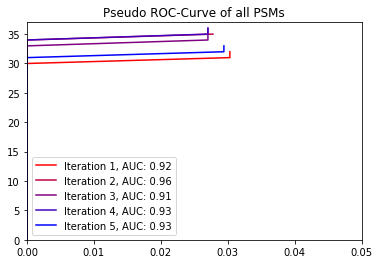
\includegraphics[width = 0.49\textwidth]{figures/badPseudoROC.png}
	\caption[Pseudo ROC of very small datasets]{The pseudo ROC curve for a Pycolator run with a small dataset. Only one decoy is included in the PSMs that count into this figure: Every PSMs with a higher score than this decoy is plotted at $0\%$~q-value, and every PSMs with a score equal or worse to the second decoy has a q-value of $\geq5\%$ and is thus not plotted.}
	\label{fig:small_dataset_pseudo_ROC}
\end{figure}
\renewcommand{\baselinestretch}{1}
A certain threshold of dataset size, for which the Percolator~algorithm gets much worse, could not be found. It gradually finds less high-confidence PSMs when the dataset size gets smaller. It is however crucial for SVM training, that there is always at least one decoy and one target PSM in every of the inner splits. This is why the algorithm returned with an error after $12$ to $93$ PSMs.\\\\
The new metric for small datasets, the number of PSMs at $1\%$~q-value, will likely not often be used, because the AUC is only not available for extremely small datasets, when Pycolator does not perform well anyways. Additionally, if the problem with the AUC on small datasets is fixed and it will always be calculated from $0$ to $5\%$, this might be a more reliable evaluation method for datasets it works on. While the number of PSMs at $1\%$~q-value might exhibit fluctuation, since the score of one decoy might make the difference if many targets obtain a q-value below or above $1\%$, this is not the case in datasets this metric is intended for. In these, a target either has a q-value of~$0$ or above~$5\%$ and is ranked higher than any decoy. While this ignores the slight inaccuracy this method of FDR estimation has (since estimating a q-value of $0\%$ for the target PSM directly ranked above the first decoy, but $\geq5\%$ for the one below seems unrealistic), it is not possible to achieve a more accurate estimation for small datasets with this method.\\\\% FALLS ICH SEITEN BRAUCHE: MÖGLICHKEIT DISKUTIEREN, DER SUCHMASCHINE MEHRERE DECOY DATABASES ANZUBIETEN
To prevent an overfitting to one spectrum or one peptide, experiments prohibiting the distribution of PSMs stemming from one spectrum or one peptide on training and validation splits were conducted. Because they yielded no usable results, they are not shown in detail in this thesis. For both, the results did not change, suggesting that neither PSMs with the same spectrum nor with the same peptide are significantly more similar than unrelated PSMs.\\\\
This thesis produced a working version of Percolator in python. As Fondrie and Noble, who also transferred Percolator to python and called it mokapot\footnote{\url{https://github.com/wfondrie/mokapot}}, write, this can be used to add flexibility to ones analyses. It is quite simple, for example, using another classifier than linear SVMs, since the machine learning methods from scikit-learn usually support the same arguments and attributes. Also, experiments like performing imputation are implemented conveniently with the scikit-learn library.\\
Although the experiments with smaller datasets brought no concrete findings, it confirmed the presumption that the Percolator algorithm works worse on smaller datasets.\\
Furthermore, two improvements were found to adapt Percolator to the characteristics of cross-linked PSMs: The ranking procedure and maintaining the proportions of different classes inside the splits. With these, Pycolator now finds 5518 cross-linked PSMs on the used dataset, as opposed to the re-implemented Percolator, which found 5450. A diagram of the algorithm with the added functionalities is shown in Figure~\ref{fig:pycolator}. 
\renewcommand{\baselinestretch}{0.9}
\begin{figure}
	\normalsize
	\centering
	\includegraphics[width = \textwidth, page = 3]{figures/Pycolator_diagram.pdf}
	\caption[Pycolator scheme]{A diagram of Pycolator. Additionally to the Percolator algorithm shown in Figure~\ref{fig:percolator}, the feature maintaining the proportions of classes inside the dataset, depicted as black and white halves, and the procedure of re-ranking, cropping and correctly scoring the PSMs with rank~$1$ are shown.}
	\label{fig:pycolator}
\end{figure}
\renewcommand{\baselinestretch}{1}
\section{Outlook}
Further research should first correct the FDR calculation and implement a method to calculate the AUC properly even for smaller datasets. Aside from that, trying out more flexible machine learning models like histogram-based gradient boosting classification trees could yield an even better separation of true and false PSMs. More flexible models should achieve results at least as high as when splitting the dataset for Pycolator~(\ref{fig:results:splitting_bases}), since they can learn the different characteristics of each of the splits and classify depending on for example the nucleotide a peptide was cross-linked onto. First experiments suggest that these models could detect characteristics of decoys rather than false PSMs, and thus disable a precise FDR estimation, but confirming this thesis requires further research.\\
Since redundant features often tend to worsen linear models and proteomics datasets often contain correlated scores, feature selection to remove redundancy might improve the models quality. Scikit-learn provides various methods for feature selection\footnote{\url{https://scikit-learn.org/stable/modules/classes.html?highlight=feature\%20selection\#module-sklearn.feature_selection}}, which could be implemented into Pycolator in further experiments.\\
Another method to reduce dimensionality is AdaBoost, where multiple weak models are combined into one strong one. Simultaneously, this only selects features that have a good impact on the predictive performance. Scikit-learn also provides functions for this\footnote{\url{https://scikit-learn.org/stable/modules/generated/sklearn.ensemble.AdaBoostClassifier.html}}, which could be implemented conveniently in further experiments.